% ============================================================================
% Lecture 22 (B21): Deep Surrogate Models
% Deep Learning for Solving and Estimating Dynamic Models in Economics and Finance
% Course author: Simon Scheidegger
% ============================================================================

\documentclass[aspectratio=169,11pt]{beamer}

% ---------- Theme and colors ----------
\usecolortheme{dove}
\setbeamertemplate{navigation symbols}{}
\setbeamertemplate{footline}{%
  \hfill\usebeamerfont{page number in head/foot}%
  \usebeamercolor[fg]{normal text}%
  \insertframenumber\,/\,\inserttotalframenumber\kern1em\vskip4pt}
\setbeamerfont{frametitle}{size=\huge}

% ---------- Packages ----------
\usepackage[utf8]{inputenc}
\usepackage[T1]{fontenc}
\usepackage{amsmath,amssymb,amsfonts}
\usepackage{bm}
\usepackage{graphicx}
\usepackage{tikz}
\usetikzlibrary{shapes,arrows.meta,positioning,calc,fit,backgrounds,patterns,decorations.pathreplacing}
\usepackage{pgfplots}
\pgfplotsset{compat=1.18}
\usepackage{booktabs}
\usepackage{hyperref}
\usepackage{multicol}
\usepackage{xcolor}
\usepackage{algorithm}
\usepackage{algorithmic}
\usepackage{listings}
\usepackage{pifont}

% ---------- Listings style for Python ----------
\lstset{
    language=Python,
    basicstyle=\small\ttfamily,
    keywordstyle=\color{uzhblue}\bfseries,
    commentstyle=\color{uzhgreydark}\itshape,
    stringstyle=\color{darkgreen},
    showstringspaces=false,
    breaklines=true,
    frame=none,
    xleftmargin=0pt,
    aboveskip=4pt,
    belowskip=4pt,
    escapeinside={(*@}{@*)},
}

% ---------- Custom colors ----------
\definecolor{uzhblue}{rgb}{0,0,0.5}
\definecolor{uzhgreylight}{RGB}{236,238,241}
\definecolor{uzhgreydark}{RGB}{81,86,94}
\definecolor{harvardcrimson}{RGB}{153,0,0}
\definecolor{unil@blue}{RGB}{0,140,204}
\definecolor{unil@black}{RGB}{35,31,32}
\definecolor{darkgreen}{RGB}{0,100,0}
\definecolor{darkred}{RGB}{139,0,0}
\definecolor{softblue}{RGB}{70,130,180}
\definecolor{softorange}{RGB}{230,159,0}
\definecolor{softgreen}{RGB}{0,158,115}

% ---------- Set beamer colors ----------
\setbeamercolor{frametitle}{bg=uzhgreylight, fg=uzhblue}
\setbeamercolor{title}{fg=uzhblue}
\setbeamercolor{structure}{fg=uzhblue}
\setbeamercolor{block title}{bg=unil@blue, fg=white}
\setbeamercolor{block body}{bg=uzhgreylight}
\setbeamercolor{block title alerted}{bg=darkred,fg=white}
\setbeamercolor{block body alerted}{bg=red!5}
\setbeamercolor{block title example}{bg=darkgreen,fg=white}
\setbeamercolor{block body example}{bg=green!5}
\setbeamercolor{item}{fg=unil@black}
\setbeamercolor{normal text}{fg=unil@black}

% ---------- Emphasis and hyperlinks ----------
\newcommand{\emphc}[1]{\textcolor{harvardcrimson}{#1}}
\hypersetup{colorlinks,linkcolor=harvardcrimson,urlcolor=harvardcrimson}

% ---------- Math commands ----------
\newcommand{\x}{\bm{x}}
\newcommand{\w}{\bm{w}}
\newcommand{\bb}{\bm{b}}
\newcommand{\z}{\bm{z}}
\newcommand{\W}{\bm{W}}
\newcommand{\X}{\bm{X}}
\renewcommand{\a}{\bm{a}}
\newcommand{\R}{\mathbb{R}}
\newcommand{\E}[1]{\mathbb{E}\!\left[#1\right]}
\DeclareMathOperator*{\argmin}{arg\,min}
\DeclareMathOperator*{\argmax}{arg\,max}

% ---------- Title ----------
\title[Lecture 22 (B21)]{Lecture 22 (B21): Deep Surrogate Models}
\subtitle{Pseudo-states, structural estimation, UQ, optimal policy, implied vol surfaces}
\author{Simon Scheidegger}
\institute{HEC, University of Lausanne}
\date{}
\begin{document}

% Custom command used in some "Finger Exercise" frame titles.
\providecommand{\exercisepause}{%
  \tikz[baseline=(X.base)]{\node[fill=darkgreen!80!black, text=white,
  rounded corners=2pt, inner sep=3pt, font=\scriptsize\bfseries](X){PAUSE};}}

{\setbeamercolor{background canvas}{bg=uzhgreylight}
\begin{frame}
\titlepage
\end{frame}
}

% --- About-this-lecture orientation ---
\begin{frame}{About this lecture}
\small
\begin{block}{What this lecture covers}
\begin{itemize}\itemsep2pt
  \item Why surrogates: replacing expensive simulators with cheap, differentiable models
  \item Pseudo-states: the trick that lets one network serve many use cases
  \item Application sketches: structural estimation, UQ, optimal policy, the implied vol surface
\end{itemize}
\end{block}
\begin{block}{Builds on}
\begin{itemize}\itemsep2pt
  \item Lectures 02-05 (NN basics)
  \item Lecture 12 (architecture / loss balancing)
\end{itemize}
\end{block}
\begin{block}{Leads to}
\begin{itemize}\itemsep2pt
  \item Lecture 23 (Gaussian processes as the Bayesian alternative)
  \item Lecture 26 (using a surrogate for SMM-based structural estimation)
\end{itemize}
\end{block}
\end{frame}

\begin{frame}{Outline}
\tableofcontents
\end{frame}

% ============================================================================
% PART I: DEEP SURROGATE MODELS
% ============================================================================
\section{Deep Surrogate Models}

% --- Slide 3: Motivation ---
\begin{frame}{Motivation: Why Surrogates?}
\begin{block}{The computational bottleneck}
Economic \& financial models are expensive to evaluate:
\begin{itemize}
  \item Solving Bellman equations / dynamic programming (DEQNs)
  \item PDE-based models (HJB, Black--Scholes for exotics)
  \item Monte Carlo simulations for risk measures
\end{itemize}
\end{block}

\vspace{0.3cm}
\begin{alertblock}{Key insight}
\emphc{We know the true model} --- we can generate \emph{unlimited} training data by solving the model on a design of experiments.
\end{alertblock}

\vspace{0.3cm}
\textbf{Goal:} Build a \emphc{surrogate} $\phi(\cdot\,|\,\theta_{NN})$ that approximates $f(\cdot)$ but evaluates \emph{orders of magnitude faster}.
\end{frame}

% --- Slide 4: Look-up Tables to Neural Networks ---
\begin{frame}{Look-up Tables $\to$ Neural Networks}
\begin{columns}[T]
\begin{column}{0.42\textwidth}
\textbf{Traditional:} pre-compute \& interpolate.\\[2pt]
\begin{center}
\footnotesize
\begin{tabular}{cc}
\toprule
$x$ & $\Phi(x)$ \\
\midrule
$-2.0$ & $0.0228$ \\
$-1.0$ & $0.1587$ \\
$\phantom{-}0.0$ & $0.5000$ \\
$\phantom{-}1.0$ & $0.8413$ \\
$\phantom{-}2.0$ & $0.9772$ \\
\bottomrule
\end{tabular}
\end{center}
\vspace{2pt}
{\footnotesize Example: standard normal CDF table.}
\end{column}

\begin{column}{0.55\textwidth}
\textbf{21st-century look-up table:}\\[2pt]
A neural network memorizes $\x \mapsto y$:
\[
\phi(\x_t\,|\,\theta_{NN}) \approx y_t = f(\x_t)
\]
\vspace{-4pt}
\begin{center}
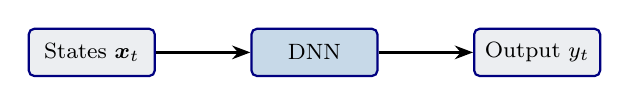
\begin{tikzpicture}[
    mlstep/.style={rectangle, draw=uzhblue, fill=uzhgreylight,
        minimum width=1.6cm, minimum height=0.6cm, font=\footnotesize,
        rounded corners=2pt, thick},
    >=Stealth
]
\node[mlstep] (input) {States $\x_t$};
\node[mlstep, right=1.2cm of input, fill=softblue!30] (dnn) {DNN};
\node[mlstep, right=1.2cm of dnn] (output) {Output $y_t$};
\draw[->, thick] (input) -- (dnn);
\draw[->, thick] (dnn) -- (output);
\end{tikzpicture}
\end{center}
\vspace{2pt}
{\footnotesize \emphc{Continuous}, \emphc{differentiable}, works in \emphc{any dimension}.}
\end{column}
\end{columns}
\end{frame}

% --- Slide 5: Pseudo-States ---
\begin{frame}{Pseudo-States: The Key Idea}
\begin{block}{Core insight (Chen, Didisheim \& Scheidegger 2026)}
Treat model parameters $\theta$ as \emphc{extra state variables}:
\vspace{-2pt}
\[
\tilde{\x} = \bigl(\underbrace{s_1,\dots,s_n}_{\text{states}},\;
\underbrace{h_1,\dots,h_h}_{\text{hidden}},\;
\underbrace{\theta_1,\dots,\theta_p}_{\text{parameters}}\bigr)
\in \R^{d}, \quad d = n + h + p.
\]
\vspace{-6pt}
\end{block}

\vspace{-0.1cm}
\begin{center}
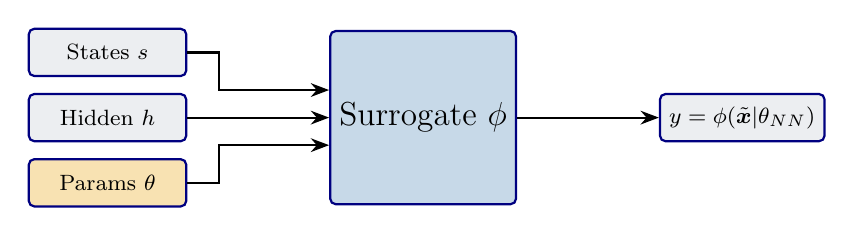
\begin{tikzpicture}[
    mlstep/.style={rectangle, draw=uzhblue, fill=uzhgreylight,
        minimum width=2cm, minimum height=0.6cm, font=\footnotesize,
        rounded corners=2pt, thick},
    >=Stealth
]
\node[mlstep] (states) {States $s$};
\node[mlstep, below=0.2cm of states] (hidden) {Hidden $h$};
\node[mlstep, below=0.2cm of hidden, fill=softorange!30] (params) {Params $\theta$};

\node[mlstep, right=1.8cm of hidden, fill=softblue!30,
      minimum width=2.2cm, minimum height=2.2cm] (surr) {\large Surrogate $\phi$};

\node[mlstep, right=1.8cm of surr] (output) {$y = \phi(\tilde{\x}|\theta_{NN})$};

\draw[->, thick] (states.east) -- ++(0.4,0) |- ([yshift=0.35cm]surr.west);
\draw[->, thick] (hidden.east) -- (surr.west);
\draw[->, thick] (params.east) -- ++(0.4,0) |- ([yshift=-0.35cm]surr.west);
\draw[->, thick] (surr) -- (output);
\end{tikzpicture}
\end{center}

\vspace{0.1cm}
Solve the model \emphc{once} over the full augmented space $\Rightarrow$ instant evaluation for \emph{any} parameter configuration.
\end{frame}

% --- Slide 6: Building the Surrogate ---
\begin{frame}{Building the Surrogate}
\begin{enumerate}
  \item \textbf{Design:} Draw $\tilde{\x}_i$ uniformly from $[\underline{x},\bar{x}]^d$, \quad $i = 1,\dots,m$.
  \item \textbf{Label:} Compute $y_i = f(\tilde{\x}_i)$ using the expensive model.
  \item \textbf{Train:} Minimize the empirical risk:
  \[
  \hat{\theta}_{NN} = \argmin_{\theta_{NN}} \frac{1}{m}\sum_{i=1}^{m}
  \bigl|\phi(\tilde{\x}_i\,|\,\theta_{NN}) - y_i\bigr|^2.
  \]
  \item \textbf{Validate:} On a held-out test set, compute max / mean absolute error.
\end{enumerate}

\vspace{0.4cm}
\begin{block}{Remark}
Since we can generate \emph{unlimited} data from the true model, the training set can be made as large as needed $\Rightarrow$ \emphc{no overfitting risk} in the traditional sense.
\end{block}
\end{frame}

% --- Slide 7: Why Surrogates Are Different ---
\begin{frame}[shrink=4]{Why Surrogates $\neq$ Standard ML}
\begin{columns}[T]
\begin{column}{0.48\textwidth}
\textbf{Standard supervised learning:}
\begin{itemize}
  \item Data is \emph{scarce} and noisy
  \item Overfitting is a major concern
  \item Regularization, early stopping, cross-validation
  \item Small learning rates, careful tuning
\end{itemize}
\end{column}
\begin{column}{0.48\textwidth}
\textbf{Surrogate modeling:}
\begin{itemize}
  \item Data is \emphc{unlimited} (we own the model)
  \item Labels are \emphc{exact} (or noise-free)
  \item Can use large epochs, aggressive LR
  \item Focus on \emph{approximation error}, not generalization
\end{itemize}
\end{column}
\end{columns}

\vspace{0.5cm}
\begin{block}{Once trained}
\begin{itemize}
  \item \emphc{Highly accurate} (errors $< 10^{-4}$ relative)
  \item \emphc{Orders of magnitude faster} than the original model
  \item \emphc{Differentiable:} gradients via automatic differentiation (backprop)
\end{itemize}
\end{block}
\end{frame}

% --- Slide 8: Speed Comparison ---
\begin{frame}{Speed Comparison: Option Pricing}
\begin{center}
{\footnotesize From Chen, Didisheim \& Scheidegger (2026), \emph{J.\ Financial Economics}:}

\vspace{0.2cm}
\small
\begin{tabular}{l r r r}
\toprule
\textbf{Task} & \textbf{FFT} & \textbf{Surr.\ (CPU)} & \textbf{Surr.\ (GPU)} \\
\midrule
Single price & $23$ ms & $\emphc{0.03}$ ms & --- \\
1-day calib.\ ($6\!\times\!10^5$) & $3.3$ h & $\emphc{18}$ s & $\emphc{0.4}$ s\\
1-year calib.\ ($1.5\!\times\!10^8$) & ${\approx}\,100$ d & $\emphc{1.2}$ h & $\emphc{98}$ s\\
\bottomrule
\end{tabular}
\end{center}

\vspace{0.3cm}
\begin{alertblock}{Takeaway}
Deep surrogates enable \emphc{real-time calibration} of option pricing models --- tasks that previously took days or were infeasible.
\end{alertblock}
\end{frame}

% --- Slide 9: Comparison of Approximation Methods ---
\begin{frame}{Comparison of Approximation Methods}
\begin{center}
\small
\begin{tabular}{l c c c c}
\toprule
\textbf{Criterion} & \textbf{Polynomials/Splines} & \textbf{Sparse Grids} & \textbf{GPs} & \textbf{DNNs} \\
\midrule
High dimension ($d > 10$) & \textcolor{darkred}{\ding{55}} & \textcolor{softorange}{$\sim$} & \textcolor{darkred}{\ding{55}} & \textcolor{darkgreen}{\ding{51}} \\
Local features / kinks    & \textcolor{darkred}{\ding{55}} & \textcolor{darkgreen}{\ding{51}} & \textcolor{softorange}{$\sim$} & \textcolor{darkgreen}{\ding{51}} \\
Irregular domains          & \textcolor{darkred}{\ding{55}} & \textcolor{darkred}{\ding{55}} & \textcolor{darkgreen}{\ding{51}} & \textcolor{darkgreen}{\ding{51}} \\
Large training set ($N > 10^4$) & \textcolor{darkgreen}{\ding{51}} & \textcolor{softorange}{$\sim$} & \textcolor{darkred}{\ding{55}} & \textcolor{darkgreen}{\ding{51}} \\
Built-in uncertainty & \textcolor{darkred}{\ding{55}} & \textcolor{darkred}{\ding{55}} & \textcolor{darkgreen}{\ding{51}} & \textcolor{darkred}{\ding{55}} \\
\bottomrule
\end{tabular}
\end{center}

\vspace{0.3cm}
\begin{itemize}
  \item \textbf{DNNs} excel in high dimensions with large data.
  \item \textbf{GPs} provide \emphc{built-in uncertainty quantification} --- crucial for active learning and Bayesian inference.
  \item \textbf{Combining both} (GP for moderate $d$ with UQ, DNN for high $d$) is a powerful strategy.
\end{itemize}
\end{frame}

% --- Slide 10: Application I — Structural Estimation ---
\begin{frame}{Application I: Structural Estimation}
\small
\textbf{Goal:} Estimate structural parameters $\theta$ from data via SMM:
\[
\hat{\theta}_{SMM} = \argmin_\theta\; [m(\theta)-\hat{m}^{\mathrm{data}}]^\top \, W \, [m(\theta)-\hat{m}^{\mathrm{data}}],
\]
where $m(\theta)$ are model-implied moments and computing them naively requires solving and simulating the model for each candidate $\theta$.

\vspace{0.15cm}
\begin{block}{Surrogate-based estimation}
\begin{enumerate}\itemsep0pt
  \item Train a surrogate policy $\phi(x,\theta)$ over \emphc{states and parameters} (pseudo-states).
  \item Reuse the trained surrogate to simulate moments $m(\theta)$ without re-solving the model.
  \item Evaluate the SMM criterion over many $\theta$ values via grid search or standard optimization.
\end{enumerate}
\end{block}

\vspace{0.15cm}
\textbf{Result:} Repeated SMM evaluations in \emphc{seconds} instead of weeks.\\
(Chen, Didisheim \& Scheidegger 2026)
\end{frame}

% --- Slide 11: Application II — Uncertainty Quantification ---
\begin{frame}{Application II: Uncertainty Quantification}
\textbf{DeepUQ} (Friedl, K\"ubler, Scheidegger \& Usui 2023):

\vspace{0.3cm}
\begin{center}
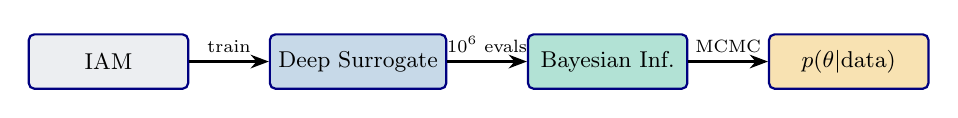
\begin{tikzpicture}[
    mlstep/.style={rectangle, draw=uzhblue, fill=uzhgreylight,
        minimum width=2.2cm, minimum height=0.75cm, font=\small,
        rounded corners=2pt, thick},
    >=Stealth, scale=0.92, transform shape
]
\node[mlstep] (model) {IAM};
\node[mlstep, right=1.1cm of model, fill=softblue!30] (surr) {Deep Surrogate};
\node[mlstep, right=1.1cm of surr, fill=softgreen!30] (bayes) {Bayesian Inf.};
\node[mlstep, right=1.1cm of bayes, fill=softorange!30] (post) {$p(\theta|\text{data})$};

\draw[->, thick] (model) -- node[above, font=\scriptsize]{train} (surr);
\draw[->, thick] (surr) -- node[above, font=\scriptsize]{$10^6$ evals} (bayes);
\draw[->, thick] (bayes) -- node[above, font=\scriptsize]{MCMC} (post);
\end{tikzpicture}
\end{center}

\vspace{0.2cm}
\begin{itemize}\small\itemsep1pt
  \item Surrogate over \emphc{100+ climate and economic parameters}
  \item Posterior distributions of \emphc{damage functions} and \emphc{optimal carbon tax}
  \item MCMC requires millions of model evaluations, only feasible with a surrogate
\end{itemize}
\end{frame}

% --- Slide 12: Application III — Optimal Policy ---
\begin{frame}{Application III: Optimal Policy}
K\"ubler, Scheidegger \& Surbek (2025):

\vspace{0.3cm}
\begin{itemize}
  \item High-dimensional integrated assessment model (IAM)
  \item \emphc{GP surrogate + Bayesian Active Learning (BAL)} for the value function
  \item GP provides \emph{uncertainty quantification} at each point
  \item BAL selects training points where uncertainty is highest
  \item Result: optimal carbon tax policy with \emphc{rigorous error bounds}
\end{itemize}

\vspace{0.3cm}
\begin{alertblock}{Preview}
Parts III and IV of this lecture introduce \emphc{Gaussian Processes} and \emphc{Bayesian Active Learning} --- the tools behind this application.
\end{alertblock}
\end{frame}

% --- Slide 12b: Application IV — Implied Volatility Surface ---
\begin{frame}{Application IV: The Implied Volatility Surface}
\textbf{Goal:} Learn the mapping from option characteristics to implied volatility.
\[
\sigma_{IV} = \phi(K, T, S_0, r, \theta_{\text{model}})
\]

\vspace{0.15cm}
\begin{center}
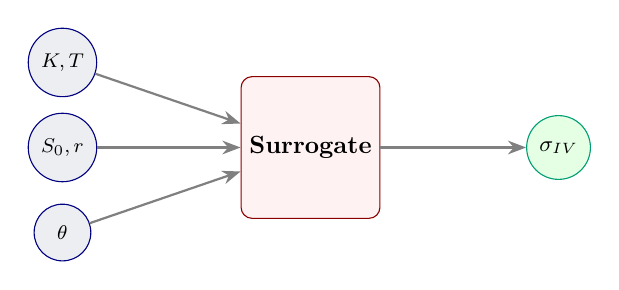
\begin{tikzpicture}[scale=0.9, transform shape,
    node distance=1.8cm,
    input/.style={circle, draw=uzhblue, fill=uzhgreylight, minimum size=0.8cm, font=\footnotesize},
    hidden/.style={rectangle, draw=darkred, fill=red!5, minimum width=1.8cm, minimum height=2cm, rounded corners},
    output/.style={circle, draw=softgreen, fill=green!10, minimum size=0.9cm, font=\small},
    arr/.style={-Stealth, thick, gray}
]
    \node[input] (K) at (0, 1.2) {$K, T$};
    \node[input] (S) at (0, 0) {$S_0, r$};
    \node[input] (P) at (0, -1.2) {$\theta$};
    \node[hidden] (net) at (3.5, 0) {\textbf{Surrogate}};
    \node[output] (IV) at (7, 0) {$\sigma_{IV}$};
    \draw[arr] (K) -- (net);
    \draw[arr] (S) -- (net);
    \draw[arr] (P) -- (net);
    \draw[arr] (net) -- (IV);
\end{tikzpicture}
\end{center}

\vspace{0.15cm}
{\small\textbf{Benefits:}
\begin{itemize}\itemsep0pt
    \item \textbf{Calibration:} Invert the surrogate to find $\theta_{\text{mod}}$ matching market prices.
    \item \textbf{Arbitrage-free:} Can enforce constraints (no calendar/butterfly arb) in the loss.
    \item \textbf{Speed:} Enables real-time pricing for complex stochastic volatility models.
\end{itemize}}
\end{frame}

% --- Slide 13: Pseudo-States — Concrete Use Cases ---
\begin{frame}{Pseudo-States: Concrete Use Cases}
\begin{block}{1. Exploring parameter distributions}
Surrogate $\phi(s, \theta)$ maps \emph{any} parameter $\theta$ to the model output instantly:
\begin{itemize}\setlength{\itemsep}{2pt}
  \item Draw $\theta^{(j)} \sim p(\theta)$ from a prior or posterior distribution
  \item Evaluate $\phi(s, \theta^{(j)})$ for each draw --- \emphc{no re-solving}
  \item Obtain the full distribution of outcomes: $\{y^{(j)}\}_{j=1}^M$
\end{itemize}
$\Rightarrow$ \emphc{Bayesian inference, sensitivity analysis, robust policy design}
\end{block}

\vspace{0.2cm}
\begin{exampleblock}{Example: Climate--economy models}
\begin{itemize}\setlength{\itemsep}{2pt}
  \item Parameters: climate sensitivity, damage curvature, discount rate
  \item Surrogate over 100+ parameters trained once ($\sim$hours)
  \item MCMC posterior with $10^6$ evaluations ($\sim$minutes with surrogate)
\end{itemize}
\end{exampleblock}
\end{frame}

% --- Slide 14: Pseudo-States — Policy Parameterization ---
\begin{frame}{Pseudo-States: Policy Parameterization}
\begin{block}{2. Parameterizing policies}
Include \emphc{policy parameters} $\theta_{\text{pol}}$ as pseudo-states.  Optimize via autograd:
\vspace{-4pt}
\[
\theta_{\text{pol}}^* = \argmax_{\theta_{\text{pol}}} \;\phi\bigl(s,\, \theta_{\text{model}},\, \theta_{\text{pol}}\bigr)
\]
\vspace{-6pt}
\end{block}

\vspace{0.1cm}
\begin{columns}[T]
\begin{column}{0.48\textwidth}
\begin{exampleblock}{Carbon tax}
\begin{itemize}\setlength{\itemsep}{0pt}
  \item Policy: tax trajectory $\theta_{\text{pol}}$
  \item Model: climate sensitivity $\theta_{\text{model}}$
  \item Optimal tax for each $\theta_{\text{model}}$
\end{itemize}
\end{exampleblock}
\end{column}
\begin{column}{0.48\textwidth}
\begin{exampleblock}{Monetary policy}
\begin{itemize}\setlength{\itemsep}{0pt}
  \item Policy: Taylor rule coefficients
  \item Model: preference / technology shocks
  \item Optimal rule via gradient descent
\end{itemize}
\end{exampleblock}
\end{column}
\end{columns}

\vspace{0.15cm}
\emphc{Key:} evaluate welfare for \emph{any} model + policy configuration instantly $\Rightarrow$ no re-solving.
\end{frame}

% --- Slide 15: Sources of Approximation Error ---
\begin{frame}{Sources of Approximation Error}
\begin{center}
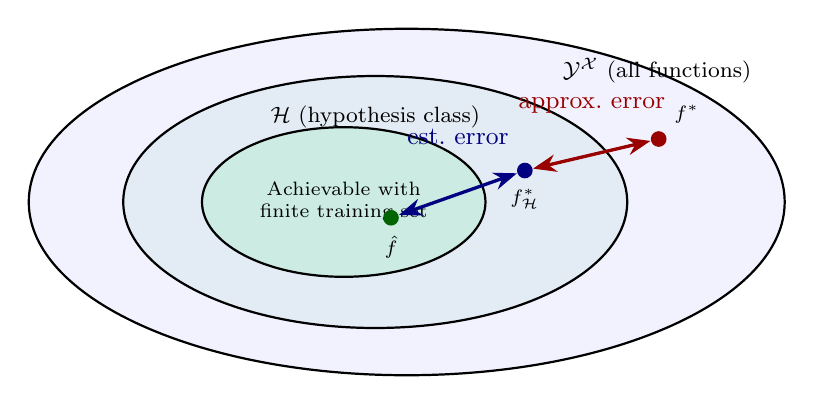
\begin{tikzpicture}[
    every node/.style={font=\footnotesize},
    >=Stealth
]
% Outer set: all functions
\draw[thick, fill=blue!5, rounded corners=8pt]
    (0,0) ellipse (4.8cm and 2.2cm);
\node[anchor=north east] at (4.5,1.95) {$\mathcal{Y}^{\mathcal{X}}$ (all functions)};

% Hypothesis class
\draw[thick, fill=softblue!15, rounded corners=6pt]
    (-0.4,0) ellipse (3.2cm and 1.6cm);
\node[anchor=north] at (-0.4,1.35) {$\mathcal{H}$ (hypothesis class)};

% Achievable with finite data
\draw[thick, fill=softgreen!20, rounded corners=4pt]
    (-0.8,0) ellipse (1.8cm and 0.95cm);
\node[font=\scriptsize, text width=2.5cm, align=center] at (-0.8,0) {Achievable with\\finite training set};

% Target function
\node[circle, fill=harvardcrimson, inner sep=2pt, label={[font=\scriptsize]above right:$f^*$}] (fstar) at (3.2,0.8) {};

% Best in H
\node[circle, fill=uzhblue, inner sep=2pt, label={[font=\scriptsize]below:$f_{\mathcal{H}}^*$}] (fH) at (1.5,0.4) {};

% Trained model
\node[circle, fill=darkgreen, inner sep=2pt, label={[font=\scriptsize]below:$\hat{f}$}] (fhat) at (-0.2,-0.2) {};

% Error arrows with readable labels
\draw[<->, very thick, harvardcrimson] (fstar) -- (fH);
\node[font=\small, text=harvardcrimson, above] at (2.35,1.0) {approx.\ error};
\draw[<->, very thick, uzhblue] (fH) -- (fhat);
\node[font=\small, text=uzhblue, above] at (0.65,0.6) {est.\ error};
\end{tikzpicture}
\end{center}

\vspace{0.1cm}
\begin{itemize}
  \item \textbf{Approximation error:} $f^*$ may not lie in $\mathcal{H}$ $\Rightarrow$ increase network capacity.
  \item \textbf{Estimation error:} finite data $\Rightarrow$ mitigated by generating more training points.
  \item For surrogates, \emphc{estimation error $\to 0$} as we can always generate more data.
\end{itemize}
\end{frame}

% --- Slide 14: Practical Tips ---
\begin{frame}{Practical Tips for Surrogate Training}
\begin{columns}[T]
\begin{column}{0.48\textwidth}
\begin{block}{Architecture}
\begin{itemize}\setlength{\itemsep}{1pt}
  \item Swish activation ($x \cdot \sigma(x)$)
  \item 3--5 hidden layers, 128--512 neurons
  \item Linear output (no activation)
\end{itemize}
\end{block}

\begin{block}{Training}
\begin{itemize}\setlength{\itemsep}{1pt}
  \item $m \geq 10^5$ samples (cheap to generate)
  \item Adam, LR $10^{-3}$, reduce on plateau
  \item Hundreds of epochs (no overfit risk)
\end{itemize}
\end{block}
\end{column}

\begin{column}{0.48\textwidth}
\begin{block}{Validation}
\begin{itemize}\setlength{\itemsep}{1pt}
  \item Held-out test set
  \item Max / mean absolute error, $R^2$
  \item Scatter: prediction vs.\ truth
\end{itemize}
\end{block}

\begin{block}{Loss functions}
\begin{itemize}\setlength{\itemsep}{1pt}
  \item MSE: $\frac{1}{m}\sum_i (\phi_i - y_i)^2$
  \item Relative $L^1$: $\frac{1}{m}\sum_i |(\phi_i - y_i)/y_i|$
\end{itemize}
\end{block}
\end{column}
\end{columns}
\end{frame}

% --- Slide 15: Summary Part I ---
\begin{frame}{Summary: Deep Surrogate Models}
\begin{enumerate}
  \item \textbf{Surrogates} = cheap, accurate replicas of expensive models.
  \item \textbf{Pseudo-states} ($\theta$ as extra inputs) unlock:
  \begin{itemize}
    \item Structural estimation (GMM in seconds)
    \item Uncertainty quantification (MCMC with surrogate)
    \item Optimal policy design
  \end{itemize}
  \item \textbf{Key advantage:} unlimited training data $\Rightarrow$ no overfitting.
  \item \textbf{Speed:} orders of magnitude faster than original model.
\end{enumerate}

\vspace{0.3cm}
\begin{block}{Hands-on}
\textbf{Notebook:} \texttt{01\_Surrogate\_Primer.ipynb} --- Black--Scholes surrogate with implied volatility inversion.
\end{block}
\end{frame}

% ============================================================================
% PART II: GAUSSIAN PROCESS REGRESSION
% ============================================================================

\end{document}
